\subsection{First definitions}
%%\mathbb{H} n'est pas introduit, c'est une notation classique dans le domaine que je ne connais pas?

To begin we will in this section give the very definition to introduce the theory of Teichmuller space

\begin{dfnt}
Let $S$ be a surface of genus $g$, a marking of $S$ is a couple $(X,f)$ made of a closed Riemann surface $X$ and of one homeomorphism $f:S \to X$ which preserve the orientation.
On the set of the marking $S$, we have a equivalence relation,  $(X_1,f_1) \sim (X_2,f_2)$ if there exist $\alpha : X_1 \to X_2 $ such that $f_2 \circ \alpha \circ f_1^{-1}$ be an homeomorphism of $S$ preserving the orientation and isotope to the identity map.%TODO diagramme
The set of the marking quotient by the previous relation is the \emph{Teichmuller space} and is written $\mathcal{T}_g$.
\end{dfnt}

\begin{rmq}
If $g \geq 2$, for every closed curve $\alpha$ of $S$, there is only one closed geodesic of $X$ freely isotope to $f(\alpha)$. Moreover if $\alpha$ is simple, so is the geodesic. We will note $l_{\alpha}(X)$ its hyperbolic length and we will take the weakest topologie on $\mathcal{T}_g$ which make this map continuous.
\end{rmq}

This give a map $L: \mathcal{T}_g \to \mathbb{R}^{\mathbf{S}}$, where $\mathbf{S}$ is the set of all simple closed curve of a given surface. We can ask if this map si injective, i.e. that a geometry is given by the length of the set of simple closed curve. The answer is yes and more precisely one can choose only $9g-9+3n$ curve so that this map is injective, as stated in Farb and Margalit (2011) Theorem 10.7. \cite{farb2011primer} %%Athé: Peut etre un peu fluidifier la lecture de la citation ?
This give the intuition that Teichmuller space can be describe only by using a finite set of parameter. We will see after that other coordinates which have nice propeties for other use.
%TODO mettre la preuve


An other curious but important fact about simple closed geodesic is that the sum of a function of theirs length is equal to a constant which does not depend on the genus or the geometry of the surface.

\begin{thm}[McShane's identity]
Let $X$ be a hyperbolic surface then \[
\sum_{\gamma} \frac{1}{1+e^{l_{\gamma}(X)}}=\frac{1}{2}
\]
Where the sum is taken over all simple closed geodesic.
\end{thm}

This theorem was proven by McShane and therefore bears his name \cite{Mcshane95simplegeodesics}. A good introduction with a proof using probablistic method on trees can be found in a paper by F. Labourie and S.P. Tan \cite{labourie:hal-01654564}.

\begin{dfnt}
The \emph{modular group} is the group of homeomorphisms of $S$ which respect orientation quotiented by the subgroup of homeomorphisms isotopic to the identity map. We will call this group $Mod_g$
It act discretely on the Teichmuller space $\mathcal{T}_g$ and the quotient is called the \emph{moduli space} and is written $\mathcal{M}_g$.
\end{dfnt}

The Teichmuller space is the universal covering of the modular space. In fact the Teichmuller space is homeomorph to a sphere and so is contractible and in particular, connected and simply connected. It is the universal covering of the moduli space.

We can ask ourselves how these spaces look and if we can give an easy representation of them. The fact is that the modular space is not manifold but an orbifold, that is a space which locally looks like a ball of a vector space quotiented by a finite group.

We will now describe objects that are natural to understand the Teichmuller space.

\begin{dfnt}
A \emph{foliation} on a surface $S$ is the collection of the following data: a finite set of points $P=(p_1,p_2,...)$, given a open covering $U_i$ on $S-P$, a collection of $C^1$
 real function $\nu_i$ such than $\| d \nu_j \| = \| d \nu_i \|$  on $U_i \cap U_j$,
 and near each singular point $p_s$ a coordinate neighborhood $V$ with complex coordinate $z$ such that $\| d \nu \| = \| Im(z^{\frac{k}{2}}dz) \|$ for some positive integer $k$ called the degree of the singular point.

 Leaves of the foliations are the graphs immersed in $S$ along which $dv$ is constant. In addition if the surface $S$  have a boundary it is required that it is contained in a singular leaf.
\end{dfnt}

The height $h_\gamma(\| d \nu \|)$ (of a free homotopy class) of a loop $\gamma$ on $S$ is the infimum in the homotopy class of the integral by $\| d \nu \|$
\[
h_\gamma(\| d \nu \|)=inf_{\gamma \sim \gamma'} \int_{\gamma'} \| d \nu \|
\]

The topology on the measured lamination that we will use is the weakest that makes the height functions continuous.

\begin{rmq}
We won't actually study the set of measured foliation but the equivalence class of \[
h_\gamma(\| d \nu \|)=h_\gamma(\| d \mu \|), \text{ for each loop } \gamma \in S
\].
We can equivalently use Whitehead equivalence relation on singular foliations by collapsing critical intervals to points and taking isotopy of foliation.
\end{rmq}

Let $\mathcal{MF}(S)$ be the space of all equivalence classes of measured foliations.
%TODO dessin et référence

\begin{dfnt}
A \emph{lamination} $\lambda$ is a closed set made of an union (non necessarily finite) of geodesics.
For each point $x$ in $\lambda$, passes only one geodesic of the lamination.
We will write this space $\mathcal{ML}(x)$.
\end{dfnt}

To understand the space of geodesic laminations it is sometimes easier to understand the "trace" of this space in the boundary circle of the universal cover of the surface. This observation gives the following definition.

\begin{dfnt}
Let $\mathcal{M}_\infty$ be the space of unordered pairs of distinct points in $\mathbb{S}^1$ \[
\mathcal{M}_\infty := \{(z,w) \in \mathbb{S}^1 \times \mathbb{S}^1 , z \neq w\}//(z,w) \equiv (w,z)
\]
Let $G$ be a discrete torsion-free group in $PSL(2,\mathbb{R})$ such that $\mathbb{H}//G=S$ is a hyperbolic surface.
A \emph{geodesic current} $\mu$ on $S$ is a $G$-invariant Radon measure on $\mathcal{M}_\infty$.
We will note $\mathcal{GC}(S)$ the space of geodesic currents, see \cite{kapovich2009hyperbolic}
\end{dfnt}

\begin{rmq}
$\mathcal{GC}(S)$ have a natural topology which is the weak $*$ convergence on continuous functions.
\end{rmq}

\begin{exmp}
Let $g \in G$ be an element that represent a simple closed geodesic on the surface $S$. The $G$-orbit of the fix point of $g$ is a discrete set on which we can put Dirac measure. This links the geodesic currents to the measured lamination.
\end{exmp}

\begin{rmq}
A multicurve is a formal sum of geodesics $\gamma = \sum a_i \gamma_i$. The space of lamination is in some aspect the closure of the set of all multicurve
\end{rmq}

\begin{dfnt}
Consider the square $\mathcal{M}_\infty^2 := \mathcal{M}_\infty \times \mathcal{M}_\infty $. In this space we can consider the open subset $\mathcal{IM}^2_\infty$ corresponding to pairs of geodesics which have transversal intersections in $\mathbb{H}$. G acts on $\mathcal{IM}^2_\infty$.
If $\mu$ and $\nu$ are geodesic currents in $\mathcal{GC}(S)$, the product $\mu \times \nu$ defines a $G$-invariant measure on $\mathcal{IM}^2_\infty$.
Finally if we take the mass of the total space $\mathcal{IM}^2_\infty // G$, the result is called the \emph{intersection number}, $i(\mu,\nu)$
\end{dfnt}

\begin{prop}
\[
i: \mathcal{GC}(S) \times \mathcal{GC}(S) \to \mathbb{R}_+
\]
is continuous and bilinear \cite{Bonahon1988}.
\end{prop}

\begin{rmq}
If $\alpha$ and $\beta$ are simple closed geodesics (Dirac measure in $\mathcal{GC}(S)$), then the intersection number is the number of intersection between $\alpha$ and $\beta$.
Actually, one can define intersection in this way, first on simple closed geodesic, then by bi-linearity on multi-curves and finally by continuity on geodesic current.
\end{rmq}

\begin{rmq}
The topology on $\mathcal{ML}$ is the weakest that make $i(.,.)$ a continuous function.
\end{rmq}

\begin{dfnt}
A \emph{quadratic differential} is a section of the square of the tangent space to $X$. It is locally as $\phi= \phi(z) dz^2$.
\end{dfnt}

\begin{rmq}
If $\phi(p) \neq 0$ we can find a map including $p$ in which $\phi = dz^2$.
Hence $\phi$ determine a flat metric on $X$ and a foliation $\mathcal{F}$ corresponding to horizontal lines.
\end{rmq}

%TODO revoir tout ca

A quadratic differential is said to be integral if\[
 \| \phi \| = \int_X | \phi | < \infty
\]
We will write $\mathcal{Q}(x)$ the Banach space of integral quadratic differentials.

\subsection{Decomposition of hyperbolic surface}

One way to construct all hyperbolic surface is to decompose them in elementary piece, that we will call pair of pant.

A hyperbolic geometric exercise shows that a hexagon which side are geodesics and with right angles is determined by the length of three sides which are not consecutive.
%QUESTION Faire cette exercice

\begin{figure}[!h]
\centering
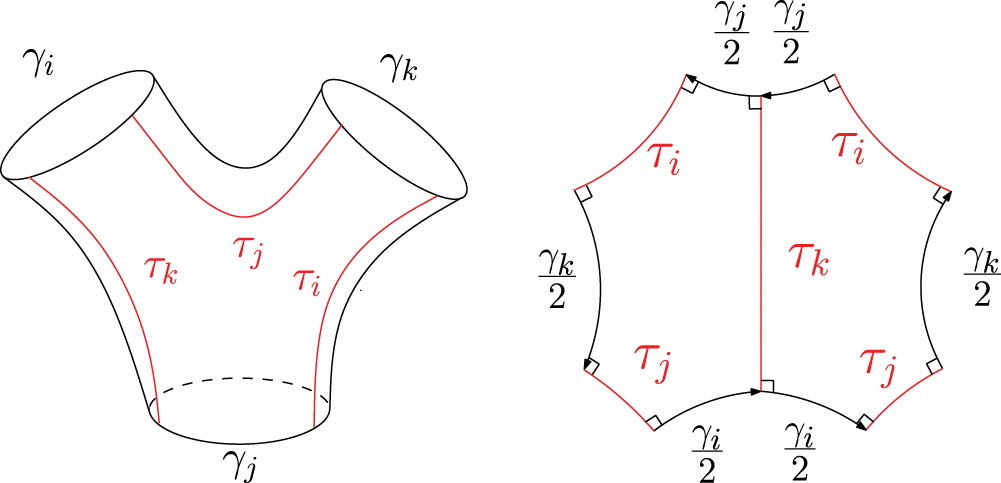
\includegraphics[width=12cm]{Image/PairOfPant.jpg}
\end{figure}

 On the image above $\gamma_i$, $\gamma_j$ and $\gamma_k$ determined the hexagon. Then we can glue them to have a pair of pant.

 \begin{dfnt}
 A \emph{pair of pant} is a hyperbolic surface with three geodesic boundaries and no punctures.
 \end{dfnt}

\begin{rmq}
The pair of pant is uniquely determined by the length of the three boundary geodesics.
\end{rmq}

\begin{proof}
As a hyperbolic polygon is uniquely determined by three non consecutive sides, the surface with boundaries that we obtain by gluing two together is determined by the length of its three boundary geodesics.
\end{proof}

\begin{rmq}
The length of one or more geodesic can go to zero and the boundaries become a puncture.
\end{rmq} %%Athé:Pas sûre du sens de la fin ? become a punctured ?

We can now decompose, with the following theorem, all hyperbolic surfaces in a collection of pair of pants.

\begin{thm}
Let $S$ be a surface of genus $g$ and with $n$ punctures. There is a set of $3g-3+n$ simple closed curves $(\gamma_1,...,\gamma_{3g-3+n})$ such that $S\ \Cup \gamma_i$ is a disjoint collection of pair of pants.
\end{thm} %%Athé je n'ai pas tout modifié, mais pour moi puncture est un nom et punctured est un adjectif... Donc n punctures ?

\begin{dfnt}
Given a surface $S$ and a pant decomposition $\gamma_1,...,\gamma_{3g-3+n}$, we have a map \[
\mathcal(S) \rightarrow (\mathbb{R^{+}}^{3g-3+n},\mathbb{R}^{3g-3+n}) \\
X \mapsto (l_{\gamma_1}(X),...,l_{\gamma_{3g-3+n}}(X),\tau_{\gamma_1}(X),...,\tau_{\gamma_{3g-3+n}}(X))
\]
This map is injective and is call the \emph{Fenchel-Nielsen} coordinates.
%TODO demontrez ça ?
\end{dfnt}

\begin{dfnt}[Dehn twist]
Let $\gamma$ be a simple closed curve. There is a tubular neighbourhood of $\gamma$ called $A$ homeomorph to $[0;1] \times S^{1}$.
A \emph{Dehn's twist} around $\gamma$ is the homeomorphism which is the identity out of $A$ and is $(t,s) \mapsto (t,e^{2i \pi t} s)$ on $A$.
\end{dfnt}

\begin{figure}[!h]
\centering
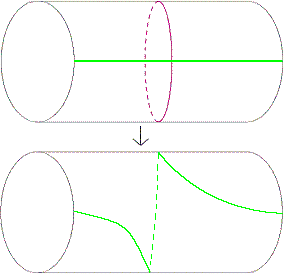
\includegraphics[width=6cm]{Image/Dehn_twist.png}
\caption{A Dehn twist}
\end{figure}

We can now give a set of generator of the modular group.

\begin{rmq}
The Lickorisk theorem states that the modular group is generated by the Dehn's twist and more precisely that one can choose only $2g+1$ generators \cite{Lickorish1964AFS}. We will give here a easier version of this theorem.
\end{rmq}

\begin{thm}
There is a collection $\delta_{1},...,\delta{9g-9}$ of simple closed curves such that $\mathcal{T}_{g} \to \mathbb{R}^{9g-9}$ is injective.
\end{thm}

\begin{proof}
Let us take $(\gamma_1,...,\gamma_{9g-9})$ a decomposition in pair of pants, let $(\alpha_1,...,\alpha_{9g-9})$ be a collection of simple closed curves such that $i(\gamma_i,\alpha_i) > 0$ and $i(\gamma_i,\alpha_j)=0$ for $i \neq j$, finally we take $\beta_i=D_{\gamma_i}(\alpha_i)$. We want to show that the length of this collection of $9g-9$ curves determined the hyperbolic structure $X \in \mathcal{T}_g$.
$X$ already has the Fenchel-Nielsen coordinate, of the pant decomposition $(\gamma_1,...,\gamma_{3g-3})$, $(l_{\gamma_1}(X),\tau_{\gamma_1}(X),...,l_{\gamma_{3g-3}}(X),\tau_{\gamma_{3g-3}}(X))$ so we need only to show that the parameters $\tau_{\gamma_i}(X)$ are determined by the length of the collection. Up to a re-normalisation we can take $\tau_{\gamma_i}(X)=0$ for every $i$. Now let's take $t=(t_1,...,t_{3g-3}) \in \mathbb{R}^{3g-3} \backslash 0$.\\
We will note $X_t$ the hyperbolic geometry which has the same length as $X$ and twist parameters $t$ in the Fenchel-Nielsen coordinate of the pair of pants. So $X_0 = X$. We will consider the function $A(t)=l_{\alpha_1}(X_t)$ and $B(t)=l_{\beta_1}(X_t)$. This function depend only of $t_1$ as $i(\gamma_i,\alpha_j)=0$ for $i \neq j$. Moreover they are strictly convex and by definition we have $A(t_1+l_(\gamma_1)(X))= B(t_1)$. We will show that there is no $t_1 \neq 0$ such that $A(t_1)=A(0)$ and $B(t_1)=B(0)$ that is $A(t_1+l_(\gamma_1)(X))=A(l_(\gamma_1)(X))$. We will note $s=t_1$ and $L=l_(\gamma_1)(X)$
Suppose there is $s \neq 0$ such that $A(s)=A(0)$, we can take $s > 0$, the other case is symmetric. If $s < L$, then by convexity for every $t \in ]0;s[$, $A(t) < A(0)=A(s)$ and $A$ is strictly increasing after $s$ so as $s < L < L+s$ we have $A(L)< A(L+s)$.
If $s > L$, then $L < s < L+s$ and  $A(L) < A(L+s)$. The final case $s=L$ is also impossible since we would have $A(0)=A(L)=A(2L)$.
Finally we can make the same argument for the other twist parameters which conclude the proof.
\end{proof}

\subsection{Flow on Teichmüller space}

We will define the main object of this document, earthquake flow.

\begin{dfnt}
The \emph{earthquake flow} is family of maps defined for $t \in \mathbb{R}$
\[
\begin{array}{crcl}

E_t: & \mathcal{ML}\times \mathcal{T}_g & \to & \mathcal{ML}\times \mathcal{T}_g \\

& (\lambda,X) & \mapsto & (\lambda,E_{t\lambda}X)

\end{array}
\]
where $E_{t \lambda}$ is first defined if $\lambda$ is a simple closed curve. In this case, we open the surface along lambda, then twist the left part of $t$ unit and put it together again. Then if $\gamma_1$ and $\gamma_2$ are two curves that don't intersect, $E_{\gamma_1}$ and $E_{\gamma_2}$ commute. So we can define the earthquake map on weighted multicurves by twisting one curve after the other by amounts proportional to the weight. Finally as multicurves are dense in the set of lamination we can extend this map for any lamination \cite{NielsenRealizationPro}.
\end{dfnt}

\begin{figure}[h!]
\centering
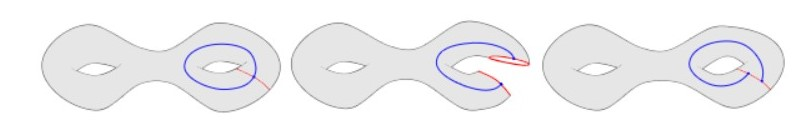
\includegraphics[width=12cm]{Image/Earthquake.jpg}
\caption{Effect of a twist on a transverse curve, image from \cite{wright2020tour}}
\end{figure}

\begin{rmq}
If the lamination is just a simple closed curve $\gamma$ then $E_{l_{\gamma}(X)}(X,\gamma)$ is just a Dehn twist around $\gamma$.
Moreover if we take a decomposition in a pair of pant that contains $\gamma$, it is just a translation in the coordinate of the twist of $\gamma$.
\end{rmq}

One could give a precise proof that the extension of the earthquake map from the multicurves to the lamination is rigorous, that is if we take two sequence $\alpha_n$ and $\alpha_n'$ of multicurves which converge to the same lamination, then the sequences of earthquake map along this multicurves converge to the same map.

We will work on universal covering of the surface, the half-plane $\mathbb{H}$
If $v \in T^1 \mathbb{H}$ we will call $\gamma(v)$ the geodesic passing by the base-point of $v$ and with $v$ as tangent vector at this point.

We have two useful lemmas to control the distortion of the earthquake map. We will not prove them, but their proofs are in \cite{NielsenRealizationPro}.

\begin{lem}\label{DisVec}
Let $l$ and $l'$ be two geodesics and $x \in l$, $y \in l'$ two points at most $\epsilon$ apart. Then if $v$ and $v'$ are the two geodesic tangents to $l$ and $l'$ respectively at point $x$ and $y$,
we have $d(v,v')<C \epsilon$ for a universal constant $C$.
\end{lem}

\begin{lem}\label{DisShe}
Let $v$ and $v'$ be two vector such that $d(v,v') < \epsilon$, let denote $\gamma=\gamma(v)$ and $\gamma'=\gamma(v')$. Let $w\in T^1 \mathbb{H}$, then \begin{enumerate}
\item $d(E_{t \gamma}w,E_{t \gamma'}w) \leq Kt \epsilon$
\item $d(E_{t \gamma}w,w) \leq Kt $
\end{enumerate}
for all $t\leq T$ and for a constant $K$ depending on $T$ and on the distance between the base-point of $v$ and $w$.
\end{lem}

With these two lemma, we can describe what happens if we change a discrete lamination by a simple closed curve that average it.

\begin{lem}
Let $x,y \in \mathbb{H}$, $v\in T_1 \mathbb{H}$ based at $y$, $\bar{A}$ the geodesic from $x$ to $y$. Suppose $\gamma$ is a discrete lamination with equal measure on each leaf whose intersection with $\bar{A}$ is included in a subarc $A$. Let $l$ be a single geodesic intersecting $A$ with angle equal to the average angle of the intersections of $\gamma$ and $A$ and with mass equal to $\mu=i(A,\gamma)$.
%TODO figure de la situation

If $A$ has length less than $\delta$ then for every $T\in \mathbb{R}^+$ the distance between $E_{t\gamma}v$ and $E_{t l}v$ is less than $Kt \mu \delta$, for all $t \leq T$ and K is a constant depending only of $T \mu$ and $d(x,y)$.
\end{lem} %%Athé: Modifié des parentheses en accolades ici  sur E_{t\gamma}v

\begin{proof}
Let denote $l_1,l_2,...,l_n$ the leaves of $\gamma$. The image of $\bar{A}$ is a disconnected arc. The point $x$ is connected to $E_{t \gamma}y$ by a staircase path going along component of $\bar{A} \backslash \gamma$ and subarc of $l_i$. Let denote the successive components $A_0,A_1,...,A_n$ and $\delta_i$ the length of $A_i$. So the staircase path is moving by $\delta_0$ along $A_0$ then by $\mu / n$ along $l_1$,and so on.

\begin{figure}[h!]
\centering
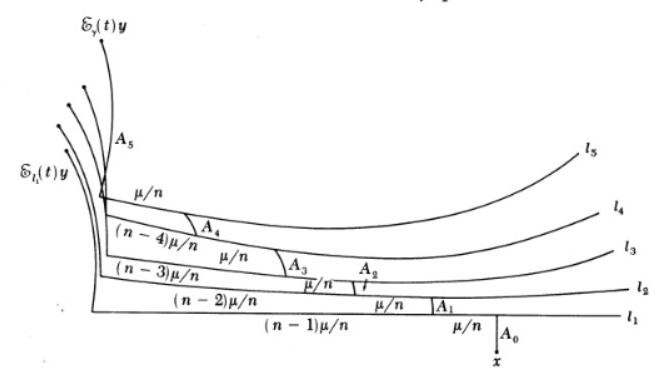
\includegraphics[width=10cm]{Image/ProofEarthquake.jpg}
\caption{Image of the construction described, image from \cite{NielsenRealizationPro}}
\end{figure}

We now alter the path by replacing the shearing along $l_n$ distance $\mu / n$ by a shearing along $l_{n-1}$ distance $2 \mu /n$. The change is less than $Kt \frac{\mu}{n}C \delta_{n-1}$ by lemma \ref{DisVec} and lemma \ref{DisShe}. Then we change the shearing by a shearing along $l_{n-2}$ of distance $3 \mu /n$ and we continue until we shear a distance $\mu$ along $l_1$. The total change is less than $KtC\sum_{i=1}^{n-1}\frac{i \mu}{n} \delta_{n-i}$
 which is less than $KCt \mu \delta$.
 We now pass from $l_1$ to $l$ with lemma \ref{DisVec} and \ref{DisShe}, and we obtain the new lemma.
\end{proof}

We need a final lemma to conclude of the well-founded definition of the earthquake flow. In this case we control the difference after earthquaking by two simple geodesic going through the same point of the arc.

\begin{lem}
Let $x$, $y$, $v$, and $\bar{A}$ be as above, if $l$ and $l'$ are geodesics of $\mathbb{H}$ with measure $\mu$ and $\mu'$ such that $l \cup \bar{A} = l' \cup \bar{A}=p \notin \{x,y\}$ and the difference between the vectors tangent of $l$ and $l'$ at $p$ of length $\mu$ and $\mu'$ is less than
$\epsilon$.

Then for any $T$, $d(E_{t l}v,E_{t l'}v)<Kt \epsilon $, for $t \leq T$ and $K$ a constant which depends only on $d(x,y)$ and $T \mu$
\end{lem}

Finally this give the theorem which control the distance between two earthquake paths.

\begin{prop}
Let $\nu \in \mathcal{ML}$ be a lamination and let $x$, $y$ be in $\mathbb{H}$, $A$ be the geodesic from $x$ to $y$ and $v\in T^1 \mathbb{H}$ be based at $y$, and $x$ and $y$ do not lie on the atomic part of $\nu$. Then for any $\epsilon$, $T$, there is a neighbourhood $U$ of $\nu$ in $\mathcal{ML}$ such that for all
$\gamma$, $\bar{\gamma}$ weighted multicurve in $U$, $d(E_{t \gamma}v,E_{t \bar{\gamma}}v) < K t \epsilon$, for all $t \leq T$, $K$ a constant depending only on $d(x,y)$ and $T i(\nu,A)$
\end{prop}

%TODO a finir si on a le temps

\begin{cor}
The earthquake flow is well defined along any lamination $\nu \in \mathcal{ML}$ and for all time $t$.
\end{cor}

\begin{rmq}
The earthquake flow is an isometry outside the support of the lamination and is continuous outside the atomic part, i.e. the simple closed geodesics of the lamination.
\end{rmq}

Thurston show that given two point in the Teichmüller space, there is a lamination $\lambda$ such that the earthquake flow from one point with respect to $\lambda$ reach the other point (also in \cite{NielsenRealizationPro}).

We can ask ourselves what is an invariant measure of this flow.

\begin{dfnt}
The \emph{Weil-Peterson form} is the form \[
\omega_{WP} = \sum d l_i \wedge d \tau_i
\]
Where $(l_1,...,\tau_1)$ are the Fenchel-Nielsen according to a pant decomposition.

This induces a measure $\mu_{WP}$.
\end{dfnt}

There is a finite measure $\nu_g$ in the Lebesgue measure class on $\mathcal{P}^1 \mathcal{M}_g$ which is invariant under the earthquake flow. This measure projects to the volume form given by $B(X) \times \mu_{WP}$ on $\mathcal{M}_g$, where \[
B(X)=\mu_{Th}(\lambda \in \mathcal{ML}, l_\lambda(X) \leq 1)
\]

There are two other important flows, the geodesic flow and the horocyclic flow.
First there is a natural homeomorphism between $T^1 \mathbb{H}  \simeq SL_2(\mathbb{R}) / SO_2(\mathbb{R})$, since $SL_2(\mathbb{R}) / SO_2(\mathbb{R})$ act simply transitively on it. This morphism can be chosen up to a conjugation via an other element of $SL_2(\mathbb{R}) / SO_2(\mathbb{R})$. We we will be interested in a special kind of subgroup.

\begin{dfnt}
A \emph{fuchsian group} $\Gamma$ is a finitely generated and discrete subgroup of $SL_2(\mathbb{R})$. Then $\Gamma$ acts discontinuously on $\mathbb{H}$.
\end{dfnt}

A Hyperbolic surface can be represented as $\mathbb{H}/ \Gamma = SL_2(\mathbb{R}) / SO_2(\mathbb{R}) / \Gamma$. If $U$ is a one parameter subgroup of $SL_2{\mathbb{R}}$ it acts on the quotient.

There are two important example:

\begin{dfnt}
The \emph{geodesic flow} is a flow on the Teichmuller space given by the action of the diagonal matrices\[
u_t=\begin{pmatrix}
e^t & 0 \\
0 & e^{-t}
\end{pmatrix}
\]
\end{dfnt}

\begin{dfnt}
The \emph{horocycle flow} is a flow on the bundle of non-zero quadratic differential, $\mathcal{QD}$, of the Teichmuller space given by the unipotent action of \[
u_t=\begin{pmatrix}
1 & t \\
0 & 1
\end{pmatrix}
\]
\end{dfnt}

The geodesic flow is also the flow that we obtain by following geodesic line on $\mathbb{H}$ and the horocycle is the flow we obtain by following curves which are everywhere orthogonal to the geodesic, which is the horizontal line and the circle tangent to the real line.

%\begin{figure}[h!]
%\centering
%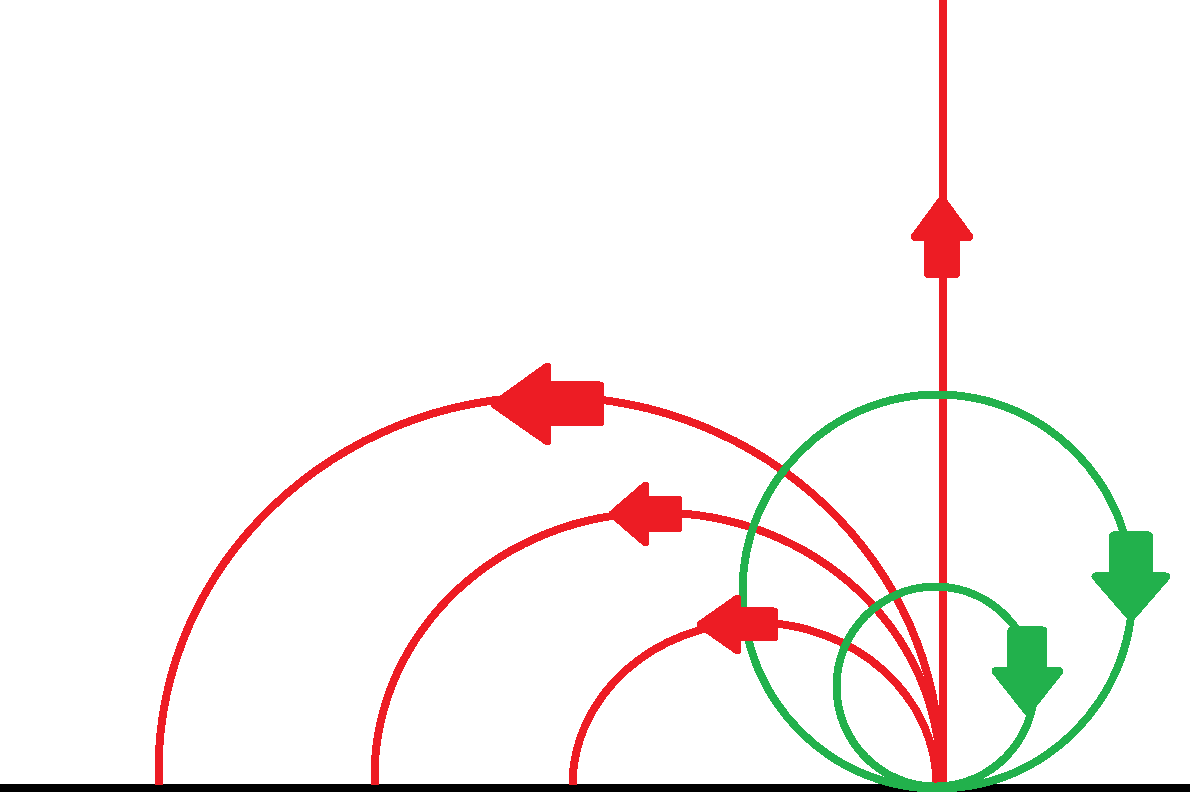
\includegraphics[width=6cm]{Image/FlowPaint.png}
%\caption{Representation of the horocycle flow, in green, and the geodesic flow, in red}
%\end{figure}



\begin{figure}
\centering
\begin{tikzpicture}[scale=1,cap=round]
\tkzInit[xmin=-6, xmax=3, ymin=0, ymax=5]
\tkzClip
%Draw circle
\tkzDefPoint(0,0){O} %define origin
\tkzDefPoint(0,1.25){C1} %define center circle 1
\tkzDefPoint(0,2){C2} %define center circle 2
\tkzDefPoint(-1,0){C3} %define center circle 3
\tkzDefPoint(-1.75,0){C4} %define center circle 4
\tkzDefPoint(-2.5, 0){C5} %define center circle 5

\draw[thick, red, postaction={decorate, decoration={markings,
            mark=at position .65 with {\arrow[scale=1.5]{stealth}};}} ] (O) -- (0, 5); %vertical line
\draw[thick] (-6, 0) -- (4, 0); %horizontal line

\tkzDrawCircle[thick, green!50!gray, postaction={decorate, decoration={markings,
            mark=at position .0 with {\arrow[scale=1.5]{stealth reversed}};}}](C1,O){circle1}
\tkzDrawCircle[thick, green!50!gray, postaction={decorate, decoration={markings,
            mark=at position .0 with {\arrow[scale=1.5]{stealth reversed}};}}](C2,O){circle2}

\tkzDrawCircle[thick, red, postaction={decorate, decoration={markings,
            mark=at position .25 with {\arrow[scale=1.5]{stealth}};}}](C3,O){circle3}
\tkzDrawCircle[thick, red, postaction={decorate, decoration={markings,
            mark=at position .25 with {\arrow[scale=1.5]{stealth}};}}](C4,O){circle4}
\tkzDrawCircle[thick, red, postaction={decorate, decoration={markings,
            mark=at position .25 with {\arrow[scale=1.5]{stealth}};}}](C5,O){circle5}


%\tkzDrawPoints(O, C1, C2, T3, C3)
%\tkzLabelPoints[below](O, C1, C2, T3, C3)
\end{tikzpicture}
\caption{}
\end{figure}
 %%Athé: Faudra mettre une legende ? Allé! je le fais !

An important relation is how this two flows interact between each other \[
\begin{pmatrix} e^t & 0 \\ 0 & e^{-t}\end{pmatrix} u_t=\begin{pmatrix} 1 & s \\ 0 & 1 \end{pmatrix} \begin{pmatrix} e^{-t} & 0 \\ 0 & e^{t}\end{pmatrix}=
\begin{pmatrix} 1 & s e^{2t} \\ 0 & 1\end{pmatrix}
\]
So the the conjugation of the horocyclic flow by the geodesic one is still the horocyclic flow.

%\begin{figure}[h!]
%\centering
%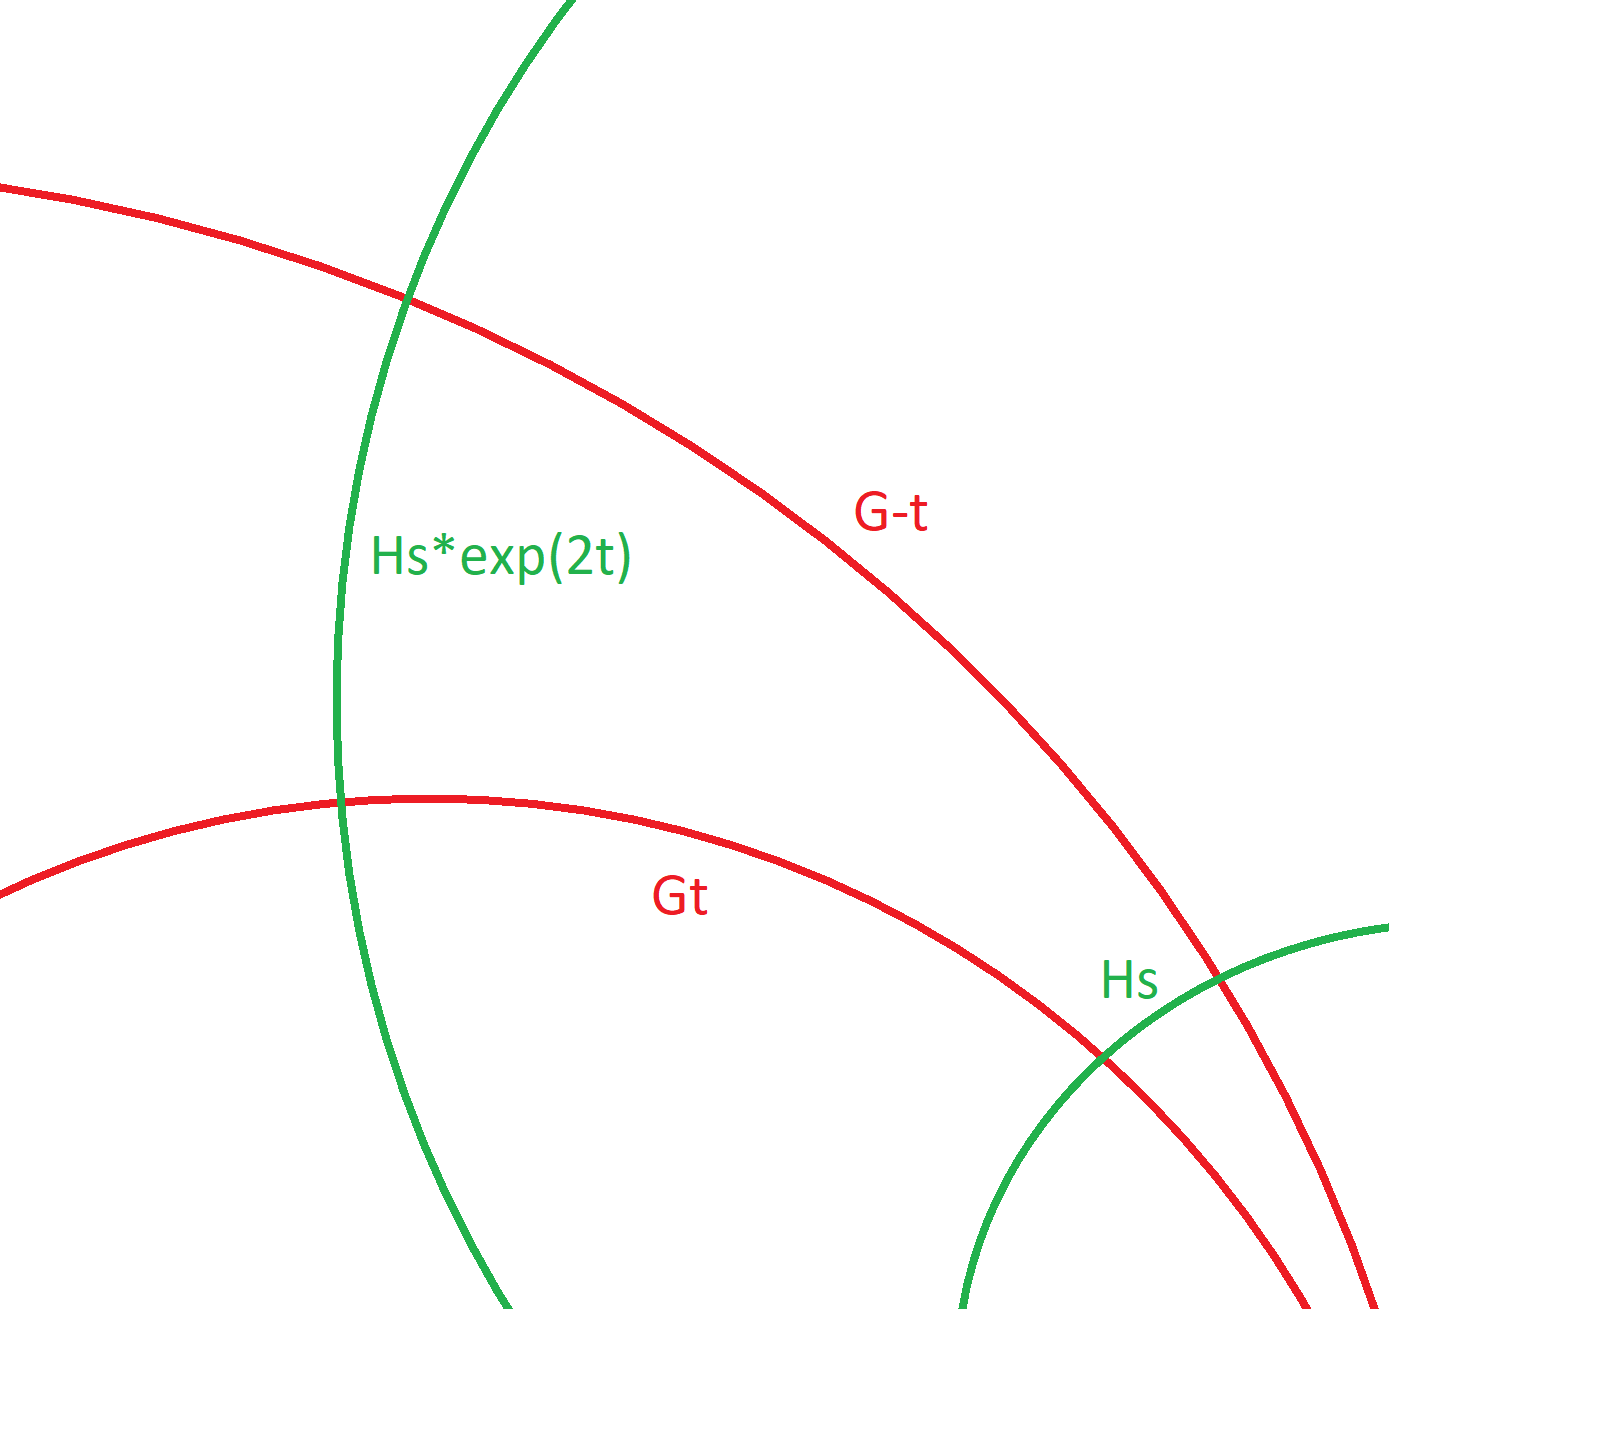
\includegraphics[width=6cm]{Image/Commutatoin.png}
%\caption{The conjugaison of the horocycle flow by the geodesic one.}
%\end{figure}

\begin{figure}
\centering
\begin{tikzpicture}[scale=1,cap=round]
\tkzInit[xmin=-7, xmax=-2.5, ymin=1.5, ymax=6]
\tkzClip
%Draw circle
\tkzDefPoint(0,0){O} %define origin
\tkzDefPoint(0,3.75){C1} %define center circle 1
\tkzDefPoint(0,6){C2} %define center circle 2
\tkzDefPoint(-3,0){C3} %define center circle 3
\tkzDefPoint(-5.25,0){C4} %define center circle 4

\tkzDrawCircle[thick, green!50!gray](C1,O){circle1}
\tkzDrawCircle[thick, green!50!gray](C2,O){circle2}

\tkzDrawCircle[thick, red](C3,O){circle3}
\tkzDrawCircle[thick, red](C4,O){circle4}

\tkzLabelPoint[shift={(-3.75cm,0.25cm)}](C1){$h_s$}
\tkzLabelPoint[shift={(-6.75cm,-2cm)}](C2){$h_{se^{2t}}$}
\tkzLabelPoint[shift={(-1.25cm,2.75cm)}](C3){$g_{t}$}
\tkzLabelPoint[shift={(0cm,5.75cm)}](C4){$g_{-t}$}

%\tkzDrawPoints(O, C1, C2, T3, C3)
%\tkzLabelPoints[below](O, C1, C2, T3, C3)
\end{tikzpicture}
\caption{The conjugaison of the horocycle flow by the geodesic one.}
\end{figure}


%QUESTION faire l'exercice du pdf sur les flots.

We give the definition of a third flow that we will use to demonstrate the ergodicity of the two previous one.

\begin{dfnt}
The \emph{rotational flow} is a flow on the bundle of nonzero quadratic differential, $\mathcal{QD}$, of the Teichmuller space given by the action of \[
e_{\theta}=\begin{pmatrix}
cos(\theta) & sin(\theta) \\
-sin(\theta) & cos(\theta)
\end{pmatrix}
\]
\end{dfnt}

We have the relation \[
h_s=e_{\theta}g_t e_{\pi+\theta}
\]

\subsection{The collaring theorem}

We will now give a useful tool to give necessary condition on length of two intersecting geodesics.

The collar function $\eta:]0; \infty[ \to ]0;\infty[$ is defined as follow. We draw a segment of length $l > 0$ on a geodesic $\gamma$, then we project perpendicularly to the geodesic the end of this segment to infinity and draw the geodesic $\delta$ which have this endpoint. So we have $\eta(l)=d(\gamma,\delta)$.

%\begin{figure}
%\centering
%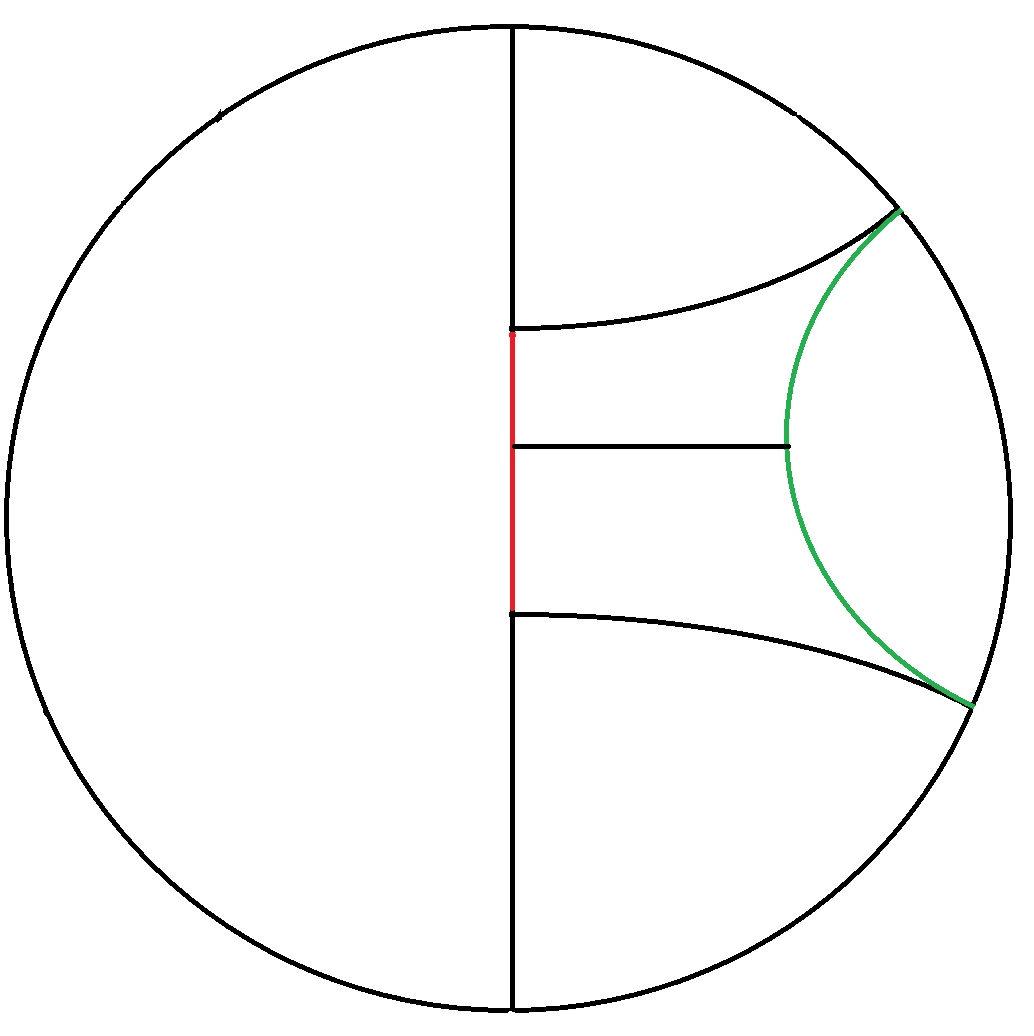
\includegraphics[width=6cm]{Image/CollarFunction.png}
%\caption{In red the segment on $\gamma$, in green $\delta$. $\eta(l)$ is the length of the black segment between them.}
%\end{figure}


%%-----------------------------
%%      the top matter
%%-----------------------------
\title{Figures}

\begin{figure}[h]
\centering
\begin{tikzpicture}[scale=1,cap=round]
\tkzInit[xmin=-4, xmax=4, ymin=-4, ymax=4]
\tkzClip
%Draw circle
\tkzDefPoint(0,0){C} %define center
\tkzDefPoint(0,4){N} %define "north"
\tkzDefPoint(0,3){NC}
\tkzDefPoint(0,-4){S} %define "south"
\tkzDefPoint(0,-2){SC}
\tkzDrawCircle[thick](C,N){circleC} %circle centered in C passing through N, named circleC
\draw[thick] (S) -- (N); %Lines between S and N

%%% North semi-arc

\tkzDefPointWith[orthogonal](NC,C) \tkzGetPoint{ortC_NC} %One point that is on the orthogonal of NC-C (passing by NC) called ortC_NC

\tkzInterLC(NC,ortC_NC)(C,N) \tkzGetPoints{N1}{N2} %The intersection between the line NC, ortC_NC and the circle centered in C passing by N, the two points are called N1 and N2

\tkzDefPointWith[orthogonal](N1,C) \tkzGetPoint{ortC_N1} %One point that is on the orthogonal of N1-C (passing by N1) called ortC_N1
\tkzDefPointWith[orthogonal](N2,C) \tkzGetPoint{ortC_N2} %One point that is on the orthogonal of N2-C (passing by N2) called ortC_N2

\tkzInterLL(N1,ortC_N1)(N2,ortC_N2) \tkzGetPoint{CN} %The intersection between the line N1-ortC_N1 and the  line N1-ortC_N1, the points is called CN

\begin{scope}
\tkzInit[xmin=0, xmax=4]
\tkzClip
\tkzClipCircle(C,N) %only what is inside the circle centered in C passing through N
\tkzDrawCircle[thick](CN,N1){circleN} %circle centered in CN passing through N1, named circleN
\end{scope}
%\tkzMarkRightAngle[size=.2](C,N2,CN)


%%% South semi-arc

\tkzDefPointWith[orthogonal](SC,C) \tkzGetPoint{ortC_SC} %One point that is on the orthogonal of SC-C (passing by SC) called ortC_SC


\tkzInterLC(SC,ortC_SC)(C,S) \tkzGetPoints{S1}{S2} %The intersection between the line SC, ortC_SC and the circle centered in C passing by S, the two points are called S1 and S2


\tkzDefPointWith[orthogonal](S1,C) \tkzGetPoint{ortC_S1} %One point that is on the orthogonal of S1-C (passing by S1) called ortC_S1
\tkzDefPointWith[orthogonal](S2,C) \tkzGetPoint{ortC_S2} %One point that is on the orthogonal of S2-C (passing by N2) called ortC_S2

\tkzInterLL(S1,ortC_S1)(S2,ortC_S2) \tkzGetPoint{CS} %The intersection between the line S1-ortC_S1 and the  line S1-ortC_S1, the points is called CS

\begin{scope}
\tkzInit[xmin=0, xmax=4]
\tkzClip
\tkzClipCircle(C,S) %only what is inside the circle centered in C passing through S
\tkzDrawCircle[thick](CS,S1){circleS} %circle centered in CS passing through S1, named circleS
\end{scope}
%\tkzMarkRightAngle[size=.2](C,S1,CS)


%%% East semi arc
\tkzInterLL(S1,ortC_S1)(N2,ortC_N2) \tkzGetPoint{CE} %The intersection between the line S1-ortC_S1 and the  line S1-ortC_S1, the points is called CS
\begin{scope}
\tkzClipCircle(C,S) %only what is inside the circle centered in C passing through S
\tkzDrawCircle[thick,green](CE,S1){circleE} %circle centered in CN passing through N1, named circleE
\end{scope}
\tkzMarkRightAngle[size=.2](C,N2,CE)
\tkzMarkRightAngle[size=.2](C,S1,CE)


\tkzDefLine[orthogonal=through CE](N,S)\tkzGetPoint{X}
\tkzInterLC(CE,X)(CE,S1) \tkzGetFirstPoint{M}
\tkzInterLL(M,X)(C,N) \tkzGetPoint{CM} %The intersection between the line SC, ortC_SC and the circle centered in C passing by S, the two points are called S1 and S2

\draw[>=triangle 45, <->, thick] (CM) -- node[below] {$\eta(\ell)$} (M);

\tkzInterLC(N,S)(CN,N1) \tkzGetSecondPoint{NM}
\tkzInterLC(N,S)(CS,S1) \tkzGetFirstPoint{SM}
\draw[>=triangle 45, <->, red, thick] (NM) -- node[left] {$\ell$} (SM);

% Mark right angles with vertical
\tkzDefPointWith[orthogonal](SM,SC)\tkzGetPoint{SME}
\tkzMarkRightAngle[size=.2](CS,SM,SME)
\tkzDefPointWith[orthogonal,K=-1](NM,NC)\tkzGetPoint{NME}
\tkzMarkRightAngle[size=.2](CN,NM,NME)

%\tkzDrawPoints(C, N, S, S1, N1, S2, N2, X, M, CM)
%\tkzLabelPoints[below](C, N, S, S1, N1, S2, N2, X, M, CM)
\end{tikzpicture}
\caption{In red the segment of length $l$ and in green the geodesic whose endpoint are orthogonal projection of the end of the segment.}
\end{figure}




It is an exercise to show that:\[
\eta(l)= \frac{1}{2} ln(\frac{cosh(l/2)+1}{cosh(l/2)-1})
\]

This quantity will be the side of a long "tube" generated by a simple closed geodesic in the hyperbolic surface. We give a definition to make this a little more precise. %%Athé: Will code a long? Pas compris

\begin{dfnt}
Let $\gamma$ be a simple closed geodesic of length $l$ on a hyperbolic surface $X$. If the $\delta$-neighbourhood \[
A_\delta(\gamma):= \{ x \in X | d(x,\gamma) < \delta \}
\]
is isometric to the $\delta$-neighbourhood of the unique simple closed geodesic on the cylinder of modulus $\frac{\pi}{l}$, we say that $\gamma$ admit a \emph{$\delta$-collar}
, or that $A_\delta(\gamma)$ is the $\delta$-collar of $\gamma$.
\end{dfnt}

We can now state a useful theorem.

\begin{thm}\label{ColLem}
Let $X$ be a complete hyperbolic surface, and let $\Gamma:={\gamma_1,...}$ be a collection of disjoint simple closed geodesic, each $\gamma_i$ of length $l_i$. Then $A_{\eta(l_i)}(\gamma_i)$ are collars around the $\gamma_i$, and they are disjoint.
\end{thm}

\begin{proof}
Choose $\gamma_1$ and $\gamma_2$ and add other simple closed curve to have a maximal multicurve that includes both.
%TODO verifier ce que cela veut dire Hubbard 3.8.3
Now cutting along this curve we have a set of pair of pants so we only have to show that the $\eta(l_i)$ neighbourhood of $\gamma_i$ the boundaries of the pair of pants do not intersect each other. We cut the pair of pants along geodesics coming from a boundary $C$ and meeting the two other boundaries $A$ and $B$. We unfold this figure in the hyperbolic plane and name the side of the octagon following the figure below.

\begin{figure}[h!]
\centering
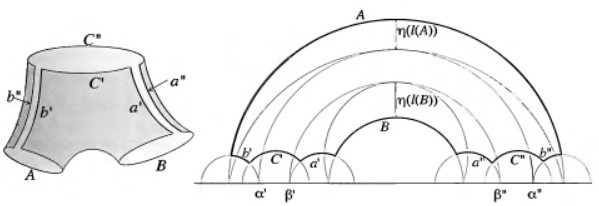
\includegraphics[width=12cm]{Image/CollarProof.jpg}
\caption{image from \cite{hubbardhal01297628}}
\end{figure}

Since $a'$ and $b'$ have the common perpendicular $C'$, they do not intersect and similarly for $a''$ and $b''$. The theorem follow easily by the definition of the function $\eta$.

\end{proof}

There are some corollaries which follow from this theorem and are ready to use in many occasions.

\begin{cor}
Let $X$ be a hyperbolic surface, and $\gamma_1$, $\gamma_2$ two simple closed geodesics on $X$ of lengths $l_1$ and $l_2$. If $l_2 < 2 \eta(l_1)$, then either $\gamma_1=\gamma_2$ or $\gamma \cap \gamma_2 = \emptyset$
\end{cor}

\begin{proof}
If $\gamma_1 \neq \gamma_2$ and $\gamma \cap \gamma_2 \neq \emptyset$ then $\gamma_2$ must cross the collar neighbourhood of $\gamma_1$ from one boundary to the other and so have length strictly superior than $2 \eta(l_1)$.
\end{proof}

\begin{cor}
Let $X$ be a hyperbolic surface, and let $\gamma_1$, $\gamma_2$ be two simple closed geodesics with lengths $< ln(3+2 \sqrt{2})$. Then either $\gamma_1=\gamma_2$ or $\gamma_1 \cap \gamma_2 = \emptyset$.
\end{cor}

\begin{cor}
Let $X$ be a complete hyperbolic surface, $\gamma$ a simple closed geodesic on $X$ of length $l$, and $A_{\gamma}$ the collar around $\gamma$. Then any simple geodesic $\delta$ on $X$ that enter $A_{\gamma}$ either intersect $\gamma$ or spirals towards $\gamma$.
\end{cor}

\begin{proof}
Suppose the geodesic $\delta$ enters $A_{\gamma}$. We can lift the situation in the universal cover of the hyperbolic disc, where $\tilde{\gamma}$ is a lift of $\gamma$ can be a diameter of the circle. Then if $\tilde{\delta}$ do not intersect $\tilde{\gamma}$
and do not have the same point at infinity, then its two endpoint are on the same side of $\tilde{\gamma}$ in the disc. Now the translation along $\tilde{\gamma}$ of length $l_{\gamma}(X)$ is in the representation of $\pi_1(X)$.
If $\tilde{\delta}$ intersect $A_{\gamma}$ then by the definition of $\delta$ it will intersect with its image by the translation cited before and hence is not simple in $X$.
\end{proof}
